\documentclass{beamer}
\usepackage[utf8]{inputenc}

\usetheme{Madrid}
\usecolortheme{default}
\useinnertheme{circles}

\definecolor{Logo1}{rgb}{0.208, 0.2865, 0.373}
\definecolor{Logo2}{rgb}{0.000, 0.674, 0.863}

\setbeamercolor*{palette primary}{bg=Logo1, fg=white}
\setbeamercolor*{palette secondary}{bg=Logo2, fg=white}
\setbeamercolor*{palette tertiary}{bg=white, fg=Logo1}
\setbeamercolor*{palette quaternary}{bg=Logo1,fg=white}
\setbeamercolor{structure}{fg=Logo1} % itemize, enumerate, etc
\setbeamercolor{section in toc}{fg=Logo1} % TOC sections

\usepackage{graphicx,animate}
%------------------------------------------------------------
%This block of code defines the information to appear in the
%Title page
\title[Linear Algebra] %optional
{Column Space \& Nullspace; Solving $Ax=0$ \& $Ax=b$}

\subtitle{Lecture 3}

\author[11910803@mail.sustech.edu.cn] % (optional)
{
    Zhang Ce
}

\institute[] % (optional)
{
    Department of Electrical and Electronic Engineering\\
    Southern University of Science and Technology
}

\date[2021.10.12] % (optional)
{2021.10.12}


%End of title page configuration block
%------------------------------------------------------------



%------------------------------------------------------------
%The next block of commands puts the table of contents at the
%beginning of each section and highlights the current section:

\AtBeginSection[]
{
\begin{frame}
    \frametitle{Table of Contents}
    \tableofcontents[currentsection]
\end{frame}
}
%------------------------------------------------------------


\begin{document}

%The next statement creates the title page.
\frame{\titlepage}


%---------------------------------------------------------
%This block of code is for the table of contents after
%the title page
\begin{frame}
\frametitle{Table of Contents}
\tableofcontents
\end{frame}
%---------------------------------------------------------
\section{A Brief Review of Last Lecture}
\begin{frame}{Last Lecture, We Discuss\dots}
Three parts in last lecture:
    \begin{enumerate}
        \item Row Exchanges and $PA=LU$ Factorization\\
        permutation matrix, process of $PA=LU$ factorization
        \item Inverse of Matrix\\
        existence of inverse, calculation of inverse, block inverse
        \item Vector Spaces and Subspaces\\
        definition of vector spaces and subspaces
    \end{enumerate}

Don't forget row method and column method for matrix multiplication. Things will get easier if you know these methods!
\end{frame}

\begin{frame}{Matrix Multiplication}
\begin{examples}
Compute the matrix multiplication.
    \begin{equation*}
        \left[ \begin{matrix}
            3&		-1&       1\\
            1&		 0&       1\\
            0&		 1&       2\\
        \end{matrix} \right] \left[ \begin{matrix}
            1&		 0&       1\\
            1&		-1&      -1\\
            1&		 2&       1\\
        \end{matrix} \right] =\left[ \begin{matrix}
            3&		 3&       5\\
            2&		 2&       2\\
            3&		 3&       1\\
        \end{matrix} \right]
    \end{equation*}
\end{examples}

\begin{enumerate}
    \item The regular (row-col) way. (Row of A) multiply (Column of B).
    \item The row way. Linear combination of (Row of B).
    \item The column way. Linear combination of (Column of A).
    \item The col-row way. (Column of A) multiply (Row of B).
\end{enumerate}

There is also an additional method: block method.
\end{frame}

\begin{frame}{Why $P^T=P^{-1}$?}
Why $P^T=P^{-1}$? A direct explanation:
\vspace{3pt}

\begin{columns}
\column{0.5\textwidth}
\begin{equation*}
    P=\left[ \begin{matrix}
        0&		1&		0&		0\\
        0&		0&		1&		0\\
        0&		0&		0&		1\\
        1&		0&		0&		0\\
    \end{matrix} \right]
\end{equation*}

\begin{itemize}
    \item 1 at $(1,2)$: (Row 2) $\rightarrow$ (Row 1).
    \item 1 at $(2,3)$: (Row 3) $\rightarrow$ (Row 2).
    \item 1 at $(3,4)$: (Row 4) $\rightarrow$ (Row 3).
    \item 1 at $(4,1)$: (Row 1) $\rightarrow$ (Row 4).
\end{itemize}

\column{0.5\textwidth}
\begin{equation*}
    P^T=\left[ \begin{matrix}
        0&		0&		0&		1\\
        1&		0&		0&		0\\
        0&		1&		0&		0\\
        0&		0&		1&		0\\
    \end{matrix} \right]
\end{equation*}

\begin{itemize}
    \item 1 at $(2,1)$: (Row 1) $\rightarrow$ (Row 2).
    \item 1 at $(3,2)$: (Row 2) $\rightarrow$ (Row 3).
    \item 1 at $(4,3)$: (Row 3) $\rightarrow$ (Row 4).
    \item 1 at $(1,4)$: (Row 4) $\rightarrow$ (Row 1).
\end{itemize}
\end{columns}

\vspace{7pt}
Exchange A and B then exchange B and A will result in exchange nothing.

\end{frame}

\begin{frame}{Existence of Inverse}
According to definition, if it has an inverse, there exist a matrix $B$ to let $AB=I$, thus, $B$ is the inverse of $A$.
\begin{equation*}
    \left[ \begin{matrix}
        1&		2\\
        3&		6\\
    \end{matrix} \right] \left[ \begin{matrix}
        x&		\cdot\\
        y&		\cdot\\
    \end{matrix} \right] =\left[ \begin{matrix}
        1&		0\\
        0&		1\\
    \end{matrix} \right]
\end{equation*}

Recall the column method of matrix multiplication:
\begin{equation*}
    x\left[ \begin{array}{c}
        1\\
        3\\
    \end{array} \right] +y\left[ \begin{array}{c}
        2\\
        6\\
    \end{array} \right] =\left[ \begin{array}{c}
        1\\
        0\\
    \end{array} \right]
\end{equation*}

It may lead you to think about column picture.

\vspace{3pt}
Linear combinations of the 2 column vectors are still on the straight line.

\vspace{3pt}
Therefore, the inverse cannot exist for this matrix $A$.

\vspace{3pt}
How about multiplying this matrix on the left side?
\end{frame}

\begin{frame}{Gauss-Jordan Method: Another Way}
\begin{example}
    Find the inverse of the following matrix:
    \begin{equation*}
        A=\left[ \begin{matrix}
            1&		2\\
            3&		7\\
        \end{matrix} \right]
    \end{equation*}
\end{example}

\textbf{Solution:}

Remember: Always do row operations.
\begin{equation*}
    \left[ \begin{matrix}
        1&		2&		1&		0\\
        3&		7&		0&		1\\
    \end{matrix} \right] \rightarrow \left[ \begin{matrix}
        1&		2&		1&		0\\
        0&		1&		-3&		1\\
    \end{matrix} \right] \rightarrow \left[ \begin{matrix}
        1&		0&		7&		-2\\
        0&		1&		-3&		1\\
    \end{matrix} \right]
\end{equation*}

Or... Column operations!
\begin{equation*}
    \left[ \begin{matrix}
        1&		2\\
        3&		7\\
        1&		0\\
        0&		1\\
    \end{matrix} \right] \rightarrow \left[ \begin{matrix}
        1&		0\\
        3&		1\\
        1&		-2\\
        0&		1\\
    \end{matrix} \right] \rightarrow \left[ \begin{matrix}
        1&		0\\
        0&		1\\
        7&		-2\\
        -3&		1\\
    \end{matrix} \right]
\end{equation*}
\end{frame}



\begin{frame}{Block Method to Find the Inverse}
\begin{example}
    Find the inverse of this matrix, given that $A,B,C$ are all invertible matrices. Please express the result in matrix form.
    \begin{equation*}
        L=\left[ \begin{matrix}
            A&		0\\
            B&		C\\
        \end{matrix} \right]
    \end{equation*}
\end{example}

\textbf{Solution:}

Core idea: Treat all block matrices as a single entry.
\begin{equation*}
    \left[ \begin{matrix}
        A&		0&		I&		0\\
        B&		C&		0&		I\\
    \end{matrix} \right] \rightarrow \left[ \begin{matrix}
        A&		0&		I&		0\\
        0&		C&		-BA^{-1}&		I\\
    \end{matrix} \right] \rightarrow \left[ \begin{matrix}
        I&		0&		A^{-1}&		0\\
        0&		I&		-C^{-1}BA^{-1}&		C^{-1}\\
    \end{matrix} \right]
\end{equation*}

\begin{equation*}
    L^{-1}=\left[ \begin{matrix}
        A^{-1}&		0\\
        -C^{-1}BA^{-1}&		C^{-1}\\
    \end{matrix} \right]
\end{equation*}

A good question to ask: why not right-multiply $C^{-1}$ in the final step?
\end{frame}

\section{Vector Spaces and Subspaces}
\begin{frame}{Vectors vs Points}
When we describe a vector, we always use arrows. But, when we describe multiple vectors, treat it as points! That is a very important concept in linear algebra.

\vspace{3pt}
Hope this video can help you establish this concept.

\vspace{8pt}

Source: The Essence of Linear Algebra -by \emph{3Blue1Brown} P3 04:44\\
\vspace{3pt}
\url{https://www.bilibili.com/video/BV1ys411472E?p=3}

\vspace{8pt}

In linear algebra, lines, planes, spaces can all be treated as a collection of vectors. That is why they are called vector spaces!

\vspace{3pt}
By the way, this series of video is really useful and can help you get a deeper understanding in linear algebra, I recommend all of you spend some time watching the first few sections after class.

\end{frame}


\begin{frame}{Subspaces of $\mathbb{R} ^2$}
Now, thing will be easier to understand the definition of vector spaces and subspaces.

\vspace{3pt}
According to definiton, a vector space inside $\mathbb{R} ^2$ is a subspace of $\mathbb{R} ^2$.

\vspace{3pt}
Try to decide whether the following ones are subspaces of $\mathbb{R} ^2$?

\begin{enumerate}
    \item $S_1=\left\{ \left( x,0 \right) |\: x\in \mathbb{R} \right\}$
    \item $S_2=\left\{ \left( x,y \right) |\: 4x+y=0 \:\&\: x,y\in \mathbb{R} \right\}$
    \item $S_3=\left\{ \left( x,y \right) |\: x+y=1 \:\&\: x,y\in \mathbb{R} \right\}$
    \item $S_4=\left\{ \left( x,y \right) |\: xy=0 \:\&\: x,y\in \mathbb{R} \right\}$\
    \item $S_5=S_1\cup S_2$
    \item $S_6=S_1\cap S_2$
    \item $S_7=\mathbb{R} ^2$
\end{enumerate}

\vspace{3pt}
A conclusion: the intersection of 2 subspaces is still a subspace, but smaller. Can you find the reason? (Use the definition to verify.)

\vspace{3pt}
Now, try to list all the subspaces for $\mathbb{R} ^2$\dots
\end{frame}

\begin{frame}{Subspaces of $\mathbb{R} ^2$}
Subspaces of $\mathbb{R} ^2$ (3 types):
\begin{enumerate}
    \item The origin. That is the zero vector $\left[ \begin{array}{c}
        0\\
        0\\
    \end{array} \right] $.
    \item Straight lines across the origin.
    \vspace{7pt}
    \item  $\mathbb{R} ^2$ itself.
\end{enumerate}

\vspace{5pt}
Can I say $\mathbb{R} ^1$? Why?

\vspace{3pt}
The vectors stored in $\mathbb{R} ^1$ have only 1 component, while the vectors in $\mathbb{R} ^2$ have 2. I have to say they are quite similar because they are both lines, but they are not the same.

\vspace{3pt}
Try to list the subspaces of $\mathbb{R} ^5$.
\end{frame}

\begin{frame}{Vector Spaces Defined from a Matrix}
Given a matrix $A$:
\begin{equation*}
    \left[ \begin{matrix}
        1&		1\\
        1&		2\\
        3&		1\\
    \end{matrix} \right]
\end{equation*}

Naturally, this matrix has 2 column vectors already:
\begin{equation*}
    \left[ \begin{array}{c}
        1\\
        1\\
        3\\
    \end{array} \right] ,\: \left[ \begin{array}{c}
        1\\
        2\\
        1\\
    \end{array} \right]
\end{equation*}

Now, find a vector space contains these 2 vectors. It is a subspace of $\mathbb{R} ^3$.

\vspace{3pt}
Which other vectors should exist in this subspace to satisfy the definition of vector spaces?

\vspace{3pt}

\end{frame}

\begin{frame}{Column Space}
To satisfy the definition of vector spaces, the scalar multiplications of those vectors (2 lines) and the addition of those vectors (the vectors between the lines) are in the final subspace. We can also say \alert{linear combinations} of the 2 vectors are in the final subspace.

\vspace{3pt}
Can you imagine the figure of this subspace? It is a 2-dimensional space across the origin in $\mathbb{R} ^3$ space. Make sure you understand it, important!
\begin{figure}
    \centering
    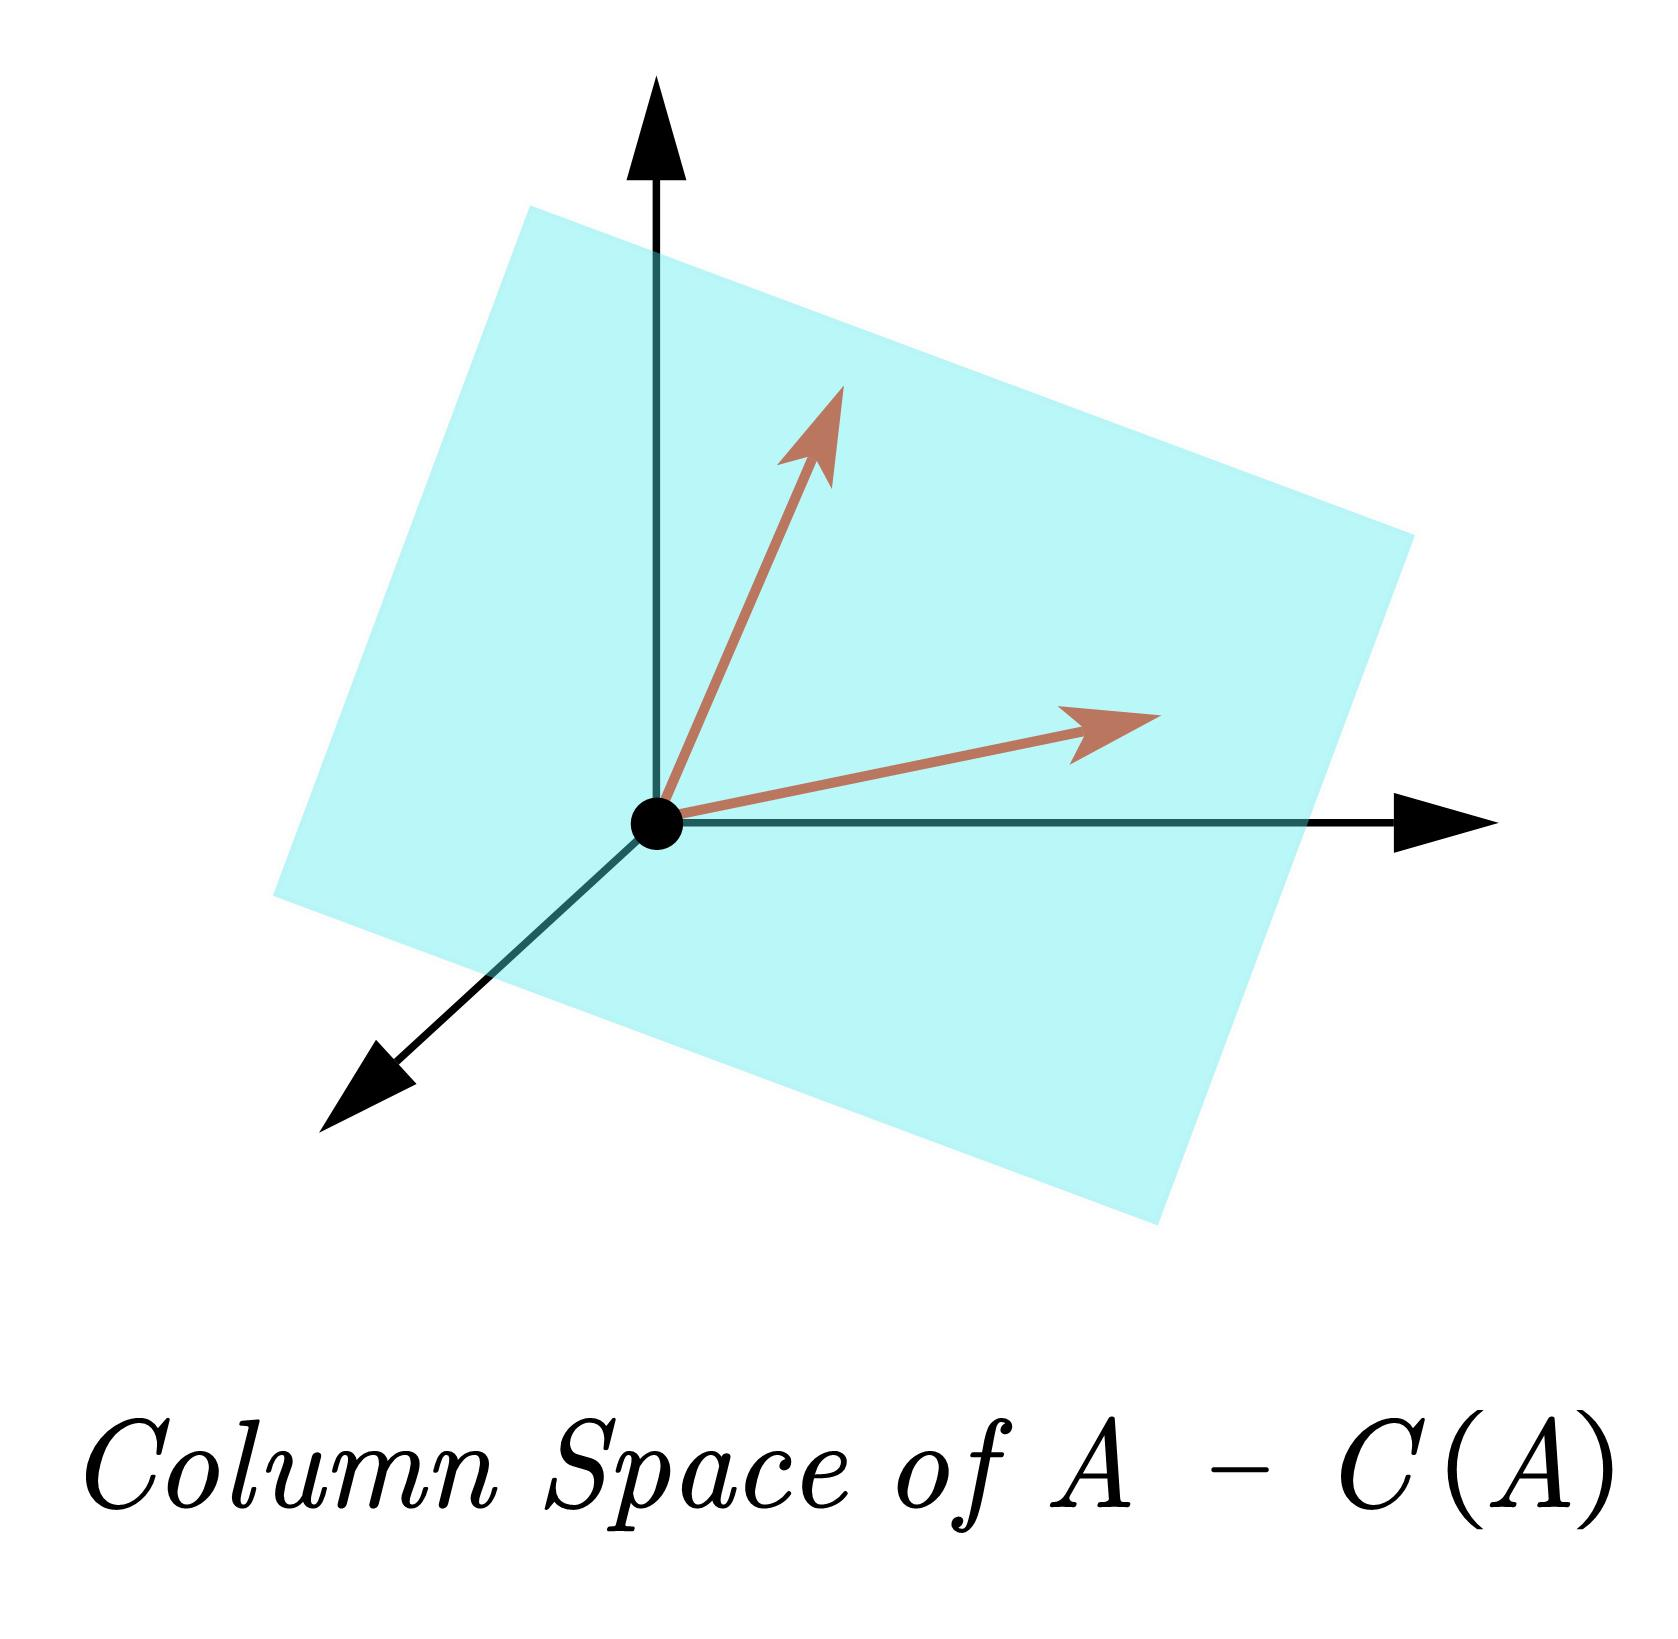
\includegraphics[width=0.3\textwidth]{column.jpg}
\end{figure}
\vspace{-14pt}
This special subspace is the column space of matrix $A$.
\end{frame}
\end{document}